% ***********************************************************
% ******************* PHYSICS HEADER ************************
% ***********************************************************
% Version 2
\documentclass[11pt]{article} 
\usepackage{amsmath} % AMS Math Package
\usepackage{amsthm} % Theorem Formatting
\usepackage{amssymb}	% Math symbols such as \mathbb
\usepackage{graphicx} % Allows for eps images
\usepackage{multicol} % Allows for multiple columns
\usepackage[dvips,letterpaper,margin=0.75in,bottom=0.5in]{geometry}
\usepackage{subfiles}
\usepackage{hyperref}
 % Sets margins and page size
\pagestyle{empty} % Removes page numbers
\makeatletter % Need for anything that contains an @ command 
\renewcommand{\maketitle} % Redefine maketitle to conserve space
{ \begingroup \vskip 10pt \begin{center} \large {\bf \@title}
	\vskip 10pt \large \@author \hskip 20pt \@date \end{center}
  \vskip 10pt \endgroup \setcounter{footnote}{0} }
\makeatother % End of region containing @ commands
\renewcommand{\labelenumi}{(\alph{enumi})} % Use letters for enumerate
% \DeclareMathOperator{\Sample}{Sample}
\let\vaccent=\v % rename builtin command \v{} to \vaccent{}
\renewcommand{\v}[1]{\ensuremath{\mathbf{#1}}} % for vectors
\newcommand{\gv}[1]{\ensuremath{\mbox{\boldmath$ #1 $}}} 
% for vectors of Greek letters
\newcommand{\uv}[1]{\ensuremath{\mathbf{\hat{#1}}}} % for unit vector
\newcommand{\abs}[1]{\left| #1 \right|} % for absolute value
\newcommand{\avg}[1]{\left< #1 \right>} % for average
\let\underdot=\d % rename builtin command \d{} to \underdot{}
\renewcommand{\d}[2]{\frac{d #1}{d #2}} % for derivatives
\newcommand{\dd}[2]{\frac{d^2 #1}{d #2^2}} % for double derivatives
\newcommand{\pd}[2]{\frac{\partial #1}{\partial #2}} 
% for partial derivatives
\newcommand{\pdd}[2]{\frac{\partial^2 #1}{\partial #2^2}} 
% for double partial derivatives
\newcommand{\pdc}[3]{\left( \frac{\partial #1}{\partial #2}
 \right)_{#3}} % for thermodynamic partial derivatives
\newcommand{\ket}[1]{\left| #1 \right>} % for Dirac bras
\newcommand{\bra}[1]{\left< #1 \right|} % for Dirac kets
\newcommand{\braket}[2]{\left< #1 \vphantom{#2} \right|
 \left. #2 \vphantom{#1} \right>} % for Dirac brackets
\newcommand{\matrixel}[3]{\left< #1 \vphantom{#2#3} \right|
 #2 \left| #3 \vphantom{#1#2} \right>} % for Dirac matrix elements
\newcommand{\grad}[1]{\gv{\nabla} #1} % for gradient
\let\divsymb=\div % rename builtin command \div to \divsymb
\renewcommand{\div}[1]{\gv{\nabla} \cdot #1} % for divergence
\newcommand{\curl}[1]{\gv{\nabla} \times #1} % for curl
\let\baraccent=\= % rename builtin command \= to \baraccent
\renewcommand{\=}[1]{\stackrel{#1}{=}} % for putting numbers above =
\newtheorem{prop}{Proposition}
\newtheorem{thm}{Theorem}[section]
\newtheorem{lem}[thm]{Lemma}
\theoremstyle{definition}
\newtheorem{dfn}{Definition}
\theoremstyle{remark}
\newtheorem*{rmk}{Remark}

% ***********************************************************
% ********************** END HEADER *************************
% ***********************************************************
\title{MITx: 8.421.1x Atomic and Optical Physics I part 1: Resonance}
\author{Piotr Kabacinski}
\begin{document}
\maketitle

\section{Resonances - an overview}

	\subsection{Introduction to resonance}
				\begin{itemize}
					\item Classical resonance - any periodic variation of some variable. When you drive a system with a variable frequency, you observe a peak at resonant frequency.
					\item Atomic Physics is interested with every single possible aspect of resonance. Resonance is the language physicists talk to atoms with.
					\item Oscillators are characterized by the sharpness of the resonance (Q - quality factor) which is a ratio of the frequency width of the resonance and its resonant frequency. Q is the number of oscillations that can be observed before the oscillation decays away.
					\item In Atomic Physics oscillators are characterized by extremely high Q factors
						\begin{itemize}
							\item optical oscillators: $10^{15}$ Hz (light frequency) $\Rightarrow$ $Q = 10^6$	(with doppler broadening), $Q = 10^{15}$ (without doppler broadening, eg. atom in optical lattice in metastable levels)
							\item mechanical oscillators: eg. quartz $Q = 10^4$ - $10^6$
							\item micromechanical oscillators: $Q = 10^5$ (eg. whispering gallery mode can have $Q = 10^9$, where light circulates around the circle of the mushroom-like structure)
							
							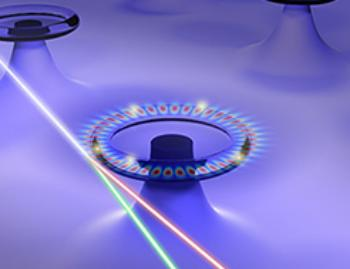
\includegraphics{whispering}
							
							\item astronomical oscillators: earth rotation: $Q = 10^7$, neutron star: $Q = 10^{10}$
						\end{itemize}
					\item "Useful" resonances are reproducible and connected by theory to fundamental constants.
					\item Rydberg constant ($R = 1.097... * 10^7 m^{-1}$) is the most accurately known constant in physics because it can be directly measured by performing spectroscopy experiments with hydrogen. Measuring fundamental constants more accurately is very important in understanding the world.
					\item Typical resonance lineshape is lorentzian which is proportional to Im$\left(\frac{1}{\omega_0-\omega+i*\frac{\gamma}{2}}\right)$. For lorentzian: $\gamma = $FWHM and $Q = \frac{\omega_0}{\gamma}$.
				\end{itemize}
				
	\subsection{Angular frequency units}
		\begin{itemize}
			\item All parameters should be measured in angular frequency units which are technically $\frac{rad}{s}$, sometimes we use $s^{-1}$. Frequencies (not angular) are measured in Hz.
			\item Good manner is to write angular frequency as $\omega_0 = 2\pi*1\text{MHz} = 6.28 * 10^6 s^{-1}$, \emph{NEVER} $6.28 * 10^{6}$ Hz.
			\item Units for $\gamma$ (temporal decay rate, inverse of dumping time) are $s^{-1}$ (\emph{NOT} Hz).
		\end{itemize}
		
\section{Resonance widths and uncertainty relations}
	\subsection{How precisely can you measure frequencies?}
		\begin{itemize}
			\item Some of the most accurate experiments in physics are done by measuring frequency.
			\item For oscillator oscillating for time $\Delta t$ with finite width of frequency spectrum $\Delta\omega$: $\Delta\omega\Delta t \geq \frac{1}{2}$
		\end{itemize}
	\subsection{Heisenberg limits on quantum and classical systems}
		\begin{itemize}
			\item kupa
		\end{itemize}
\end{document}